\documentclass[10pt,executivepaper]{article}
\usepackage[utf8]{inputenc}
\usepackage[spanish]{babel}
\usepackage{amsmath}
\usepackage{amsfonts}
\usepackage{amssymb}
\usepackage{graphics}
\usepackage{graphicx}
\usepackage[left=2cm,right=2cm,top=2cm,bottom=2cm]{geometry}
\usepackage{imakeidx}
\makeindex[columns=3, title=Alphabetical Index, intoc]
\usepackage{listings}
\usepackage{xcolor}
\usepackage{multicol}
\usepackage{changepage}
\usepackage{float}
\usepackage{cite}
\usepackage{url}
\usepackage{pdflscape}
\usepackage{listingsutf8}

\definecolor{codegreen}{rgb}{0,0.6,0}
\definecolor{codegray}{rgb}{0.5,0.5,0.5}
\definecolor{codepurple}{rgb}{0.58,0,0.82}
\definecolor{backcolour}{rgb}{0.95,0.95,0.92}

\lstdefinestyle{mystyle}{
    backgroundcolor=\color{backcolour},
    commentstyle=\color{codegreen},
    keywordstyle=\color{magenta},
    numberstyle=\tiny\color{codegray},
    stringstyle=\color{codepurple},
    basicstyle=\ttfamily\footnotesize,
    breakatwhitespace=false,
    breaklines=true,
    captionpos=b,
    keepspaces=true,
    numbers=left,
    numbersep=5pt,
    showspaces=false,
    showstringspaces=false,
    showtabs=false,
    tabsize=3,
    inputencoding=utf8,
    extendedchars=true,
    literate={á}{{\'a}}1 {ñ}{{\~n}}1 {é}{{\'e}}1,
}

\def\fillandplacepagenumber{%
 \par\pagestyle{empty}%
 \vbox to 0pt{\vss}\vfill
 \vbox to 0pt{\baselineskip0pt
   \hbox to\linewidth{\hss}%
   \baselineskip\footskip
   \hbox to\linewidth{%
     \hfil\thepage\hfil}\vss}}


\lstset{style=mystyle}

\title{Actividad: Replicación de un servidor en la nube}

\author{Instituto Politécnico Nacional\\Escuela Superior de Computo\\Desarrollo de Sistemas Distribuidos\\Adrian González Pardo\\4CV1\\21/01}
\date{\today}
\newcommand\tab[1][1cm]{\hspace*{#1}}

\begin{document}
% Portada
%encabezado
\begin{minipage}{0.4\textwidth}
	\begin{flushleft}
		
\includegraphics[scale = 0.05]{logoescom.png}
	\end{flushleft}
\end{minipage}
\begin{minipage}{0.51\textwidth}
	\begin{flushright}
		
\includegraphics[scale = 0.055]{logoipn.png}
	\end{flushright}
\end{minipage}
\begin{center}
	\par\vspace{0.5cm}{
	\huge\textbf{Instituto Politécnico Nacional \\*[0.20cm] Escuela Superior de Cómputo}}
\par\vspace{1cm}{
	\large\textbf{Desarrollo de Sistemas Distribuidos\\Actividad: Replicación de un servidor en la nube\\Curso impartido por el profesor: Pineda Guerrero Carlos\\Grupo: 4CV1\\21/01\\Alumno: Adrian González Pardo\\}
}
\par\vspace{1cm}{
	
\includegraphics[scale=0.5]{servers.jpg}
}
\par\vspace{2cm}{
	Ultima fecha modificado: \today
}
\end{center}

% Indice
\clearpage
\section{Desarrollo}
Para esta tarea fue necesario hacer uso de dos maquinas virtuales con Linux y la maquina local con Windows (Winbugs), la cual debe tener instalados los archivos de las aplicaciones contenidas de Putty como \textit{putty.exe}, y \textit{psftp.exe} las cuales pueden ser trabajadas desde las variables de entorno para ser ejecutadas en cmd o en Powershell de forma más sencilla, sobre todo \textit{psftp.exe} que necesita al igual que ssh un usario y una dirección IP o de host.
\section{Códigos y scripts para funcionamiento}
\subsection{Código modificado Cliente2.java}
\lstinputlisting[language=Java]{mod.java}

Para el lado de las maquinas virtuales se hizo uso de dos scripts los cuales permiten instalar de forma rápida y sencilla todo lo que necesitaremos, pero para ejecutar estos scripts es necesario ya haber mandado todos los archivos con los que va a trabajar la maquina virtual.
\subsection{Script para VM 1}
\lstinputlisting[language=Bash]{../script1.sh}
\subsection{Script para VM 2}
\lstinputlisting[language=Bash]{../script2.sh}

\section{Capturas}
\subsection{VM}
\begin{center}
  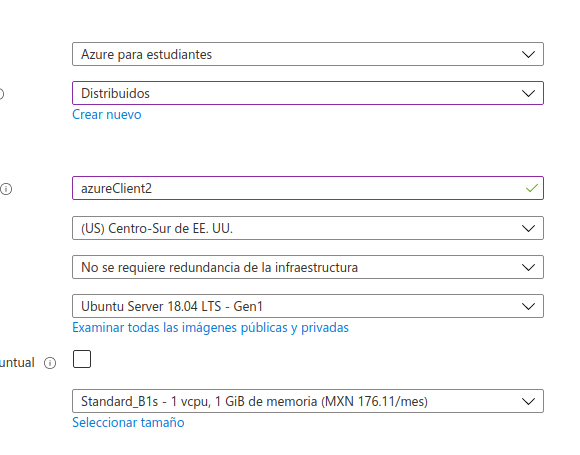
\includegraphics[scale=0.5]{imgs/creacion_0.png}\\
  \textit{Figura 1: Casillas de selección para la creación de la VM}\\
  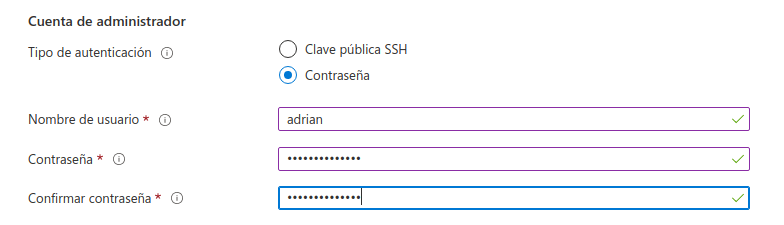
\includegraphics[scale=0.5]{imgs/creacion_1.png}\\
  \textit{Figura 2: Casillas de selección para la creación de la VM}\\
  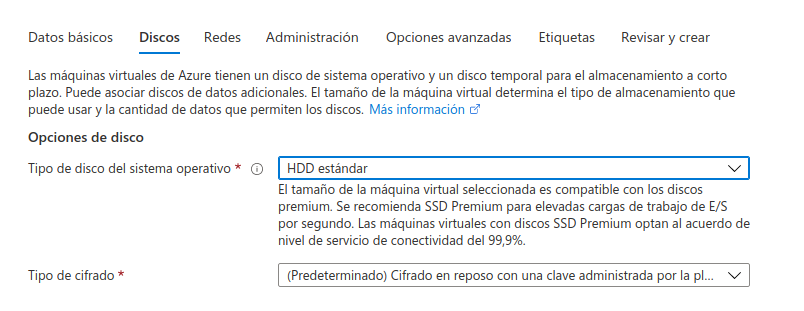
\includegraphics[scale=0.5]{imgs/creacion_3.png}\\
  \textit{Figura 3: Casillas de selección para la creación de la VM}\\
  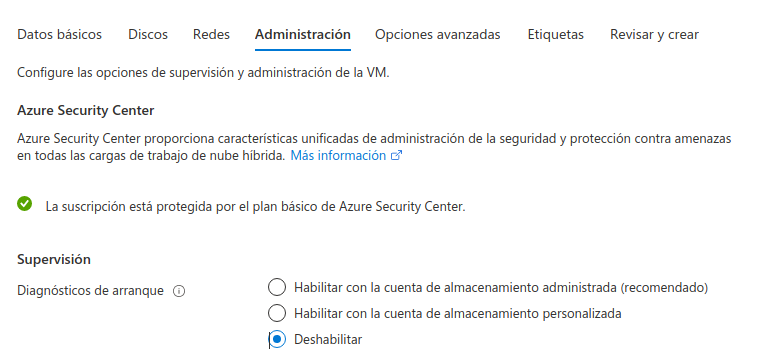
\includegraphics[scale=0.5]{imgs/creacion_4.png}\\
  \textit{Figura 4: Casillas de selección para la creación de la VM}\\
  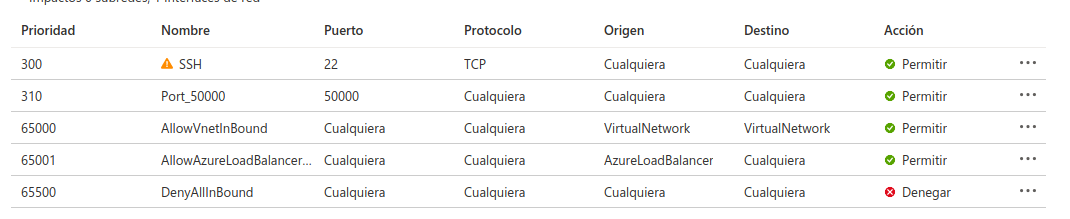
\includegraphics[scale=0.4]{imgs/config_net.png}\\
  \textit{Figura 5: Configuración de puertos para funcionamiento de la aplicación}
\end{center}
\subsection{Apartado de Winbugs}
\begin{center}
  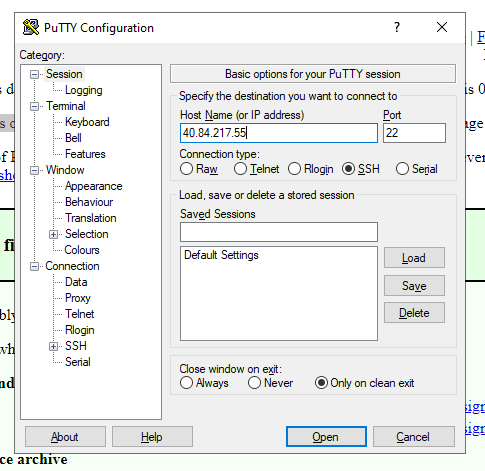
\includegraphics[scale=0.65]{imgs/putty.png}\\
  \textit{Figura 6: Conexión desde putty}\\
  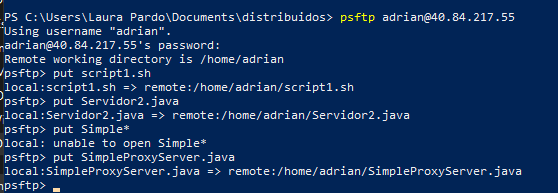
\includegraphics[scale=0.65]{imgs/conexion_psftp.png}\\
  \textit{Figura 7: Conexion de psftp desde Powershell para enviar archivos java y sh}\\
  \textbf{Para enviar archivos desde psftp solo es necesario hacer un put $<$archivo$>$}\\
  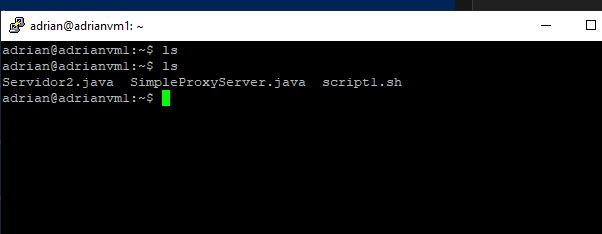
\includegraphics[scale=0.65]{imgs/envio_de_archivos.png}\\
  \textit{Figura 8: ls antes y despues de ejecutar el psftp en la maquina virtual}\\
  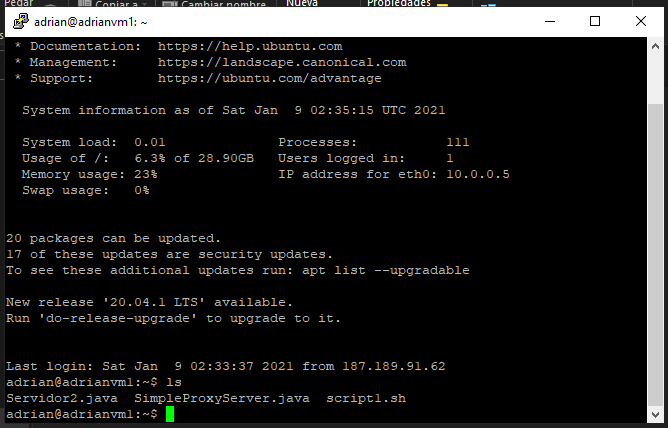
\includegraphics[scale=0.65]{imgs/vm_1.png}\\
  \textit{Figura 9: Conexion a maquina 1 desde Putty}\\
  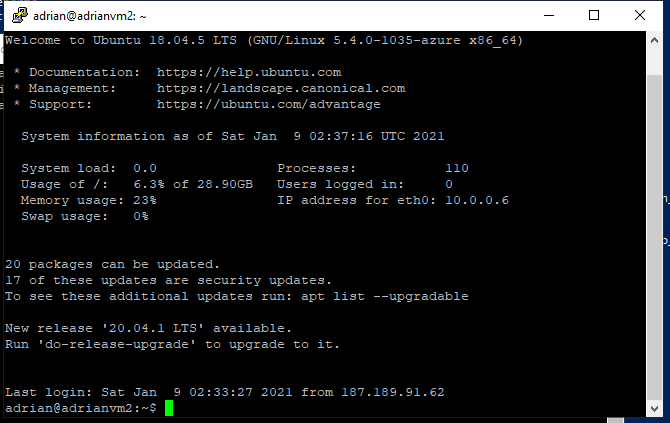
\includegraphics[scale=0.65]{imgs/vm_2.png}\\
  \textit{Figura 10: Conexion a maquina 2 desde Putty}\\
  \textbf{Despues de realizar esto es necesario primero ejecutar el script2.sh en la VM2}\\
  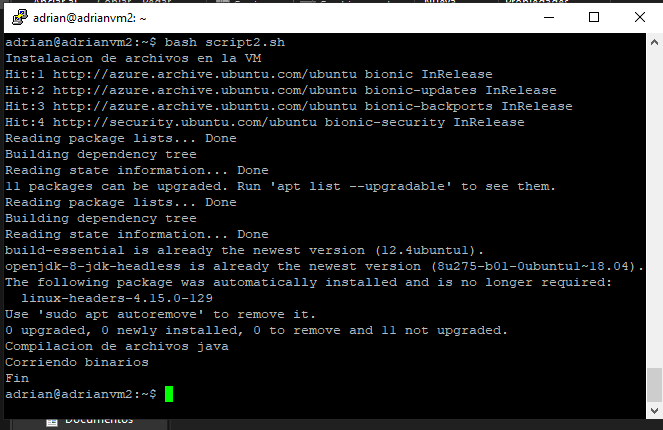
\includegraphics[scale=0.65]{imgs/vm2_ex.png}\\
  \textit{Figura 11: Ejecución del script 2 }\\
  \textbf{Despues se sigue con el script1.sh y la IP de la VM2 para su correcto funcionamiento}
  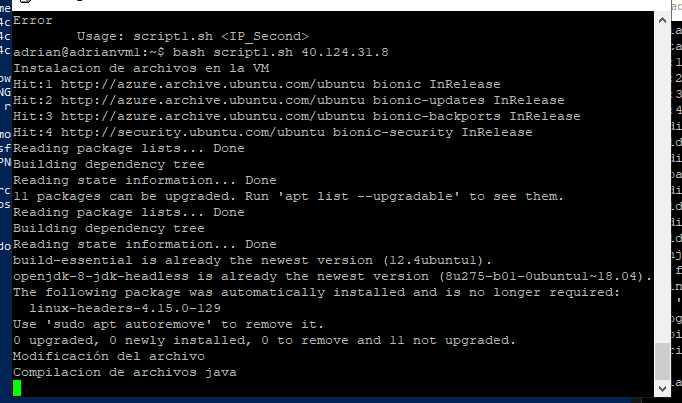
\includegraphics[scale=0.65]{imgs/vm1_ex.png}\\
  \textit{Figura 12: Ejecución del script 1}\\
  \textbf{Finalmente ejecutaremos nuestro cliente de tal modo en que pondremos la IP de la VM1}\\
  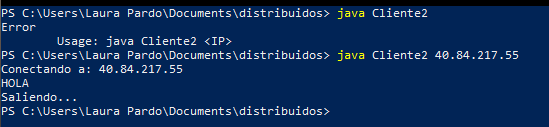
\includegraphics[scale=0.75]{imgs/ex_cliente.png}\\
  \textit{Figura 13: Ejecución del cliente}\\
  \begin{landscape}
    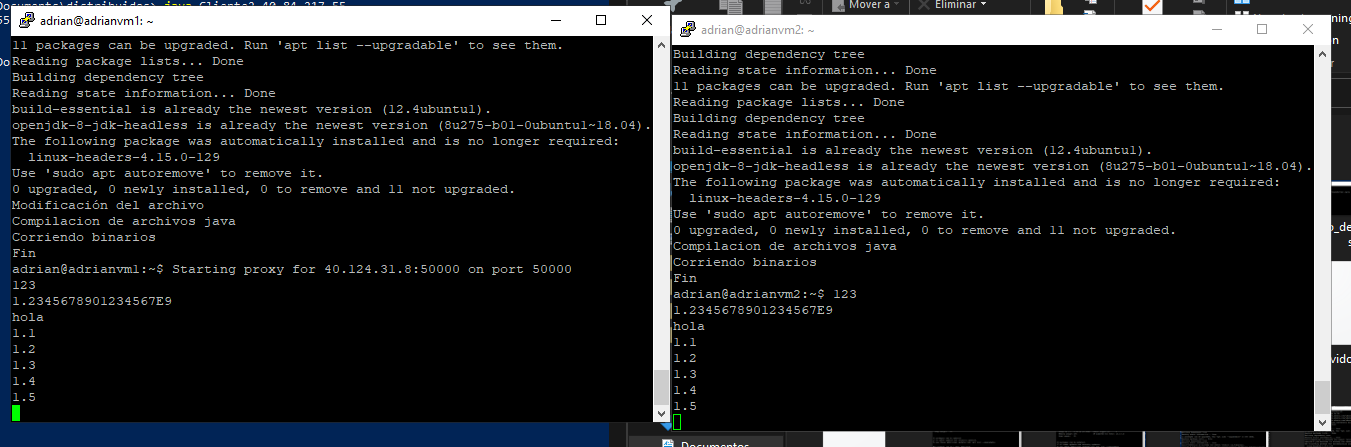
\includegraphics[scale=0.65]{imgs/ex_vms.png}\\
    \textit{Figura 14: Vistazo a los servidores o VMs de tal modo en que vemos como se replica la información.}
    \fillandplacepagenumber
  \end{landscape}
\end{center}
\section{Conclusiones}
Finalmente como podemos ver el hacer uso de servidores los cuales puedan replicar la información a traves de un proxy o de otro tipo de medio es de suma importancia ya que así se puede mantener un control de logs pensandolo en servicios web para algunos servicios que vemos generalmente como Google que tiene multiples servidores para atender las peticiones de los usuarios, o pensando en algun Webservice que funcione con este tipo de metodología, por otro lado el hacer uso de un sistema que no es Linux muchas veces no permite la creación o automatización de varios procesos mediante scripting, por lo que es necesario recurrir en algunas ocasiones a herramientas terceras como Putty, y añadir estas herramientas luego puede ser tan doloso que en Linux simplemente todo podría funcionar con unas lineas como \textit{sshpass} para evitar la parte del password, \textit{ssh} para la conexión al servidor o para la ejecución de algún comando, y \textit{scp} para mandar archivos a la maquina o viceversa.
\\\vspace{0.15cm}
\textbf{Para el caso de ser implementado via Linux los comandos o el script a ejecutar seria el siguiente:}
\lstinputlisting[language=Bash]{../script_install.sh}
\end{document}
